\documentclass[UTF8]{book}
\usepackage{ctex}

\usepackage{amssymb,amsmath,amsfonts} %公式包

\usepackage{geometry}          % 用于页面设置
\geometry{a4paper, scale=0.8}  % 设置为A4纸,边距0.8
\usepackage{graphics}          % 与图形有关

\usepackage{graphicx} % ⋯⋯导言区其他内容

\usepackage{titlesec} %设置标题类型,参照:http://blog.sina.com.cn/s/blog_94d13e7501010pye.html
\titleformat{\chapter}{\centering\Huge\bfseries}{第\,\thechapter\,章}{1em}{}


\usepackage{indentfirst}
\setlength{\parindent}{2em}

%注意,CJK和ctex包的首行缩进不一样,参见:https://www.cnblogs.com/airbird/p/LaTex_1st_line_tab.html
%\usepackage{indentfirst} %段首空两格
%\setlength{\parindent}{4pt} %设置空任意数目的

\usepackage{bibentry,natbib,plain}

\title{\textbf{从DSO来看视觉里程计}}
\author{文坤\\22}
\date{} %系统会自动生成一个时间,通过该命令取消时间显示 

\pagestyle{plain}  % 设置页码风格


%设置插入代码的风格
\usepackage{listings}
\usepackage{xcolor}

\definecolor{mygreen}{rgb}{0,0.6,0}  
\definecolor{mygray}{rgb}{0.5,0.5,0.5}  
\definecolor{mymauve}{rgb}{0.58,0,0.82}  

\usepackage{caption}
\lstset{
	language=C++,
	basicstyle=\small\ttfamily,
	numbers=left,   %行号
	numbersep=5pt,
	xleftmargin=20pt,
	frame=shadowbox,
	framexleftmargin=20pt
}
\renewcommand*\thelstnumber{\arabic{lstnumber}:}
\DeclareCaptionFormat{mylst}{\hrule#1#2#3}
\captionsetup[lstlisting]{format=mylst,labelfont=bf,singlelinecheck=off,labelsep=space}

%
%\lstset{ %  
%	backgroundcolor=\color{white},   % choose the background color; you must add \usepackage{color} or \usepackage{xcolor}  
%	basicstyle=\footnotesize,        % the size of the fonts that are used for the code  
%	breakatwhitespace=false,         % sets if automatic breaks should only happen at whitespace  
%	breaklines=true,                 % sets automatic line breaking  
%	captionpos=bl,                    % sets the caption-position to bottom  
%	commentstyle=\color{mygreen},    % comment style  
%	deletekeywords={...},            % if you want to delete keywords from the given language  
%	escapeinside={\%*}{*)},          % if you want to add LaTeX within your code  
%	extendedchars=true,              % lets you use non-ASCII characters; for 8-bits encodings only, does not work with UTF-8  
%	frame=single,                    % adds a frame around the code  
%	keepspaces=true,                 % keeps spaces in text, useful for keeping indentation of code (possibly needs columns=flexible)  
%	keywordstyle=\color{blue},       % keyword style  
%	%language=Python,                 % the language of the code  
%	morekeywords={*,...},            % if you want to add more keywords to the set  
%	numbers=left,                    % where to put the line-numbers; possible values are (none, left, right)  
%	numbersep=5pt,                   % how far the line-numbers are from the code  
%	numberstyle=\tiny\color{mygray}, % the style that is used for the line-numbers  
%	rulecolor=\color{black},         % if not set, the frame-color may be changed on line-breaks within not-black text (e.g. comments (green here))  
%	showspaces=false,                % show spaces everywhere adding particular underscores; it overrides 'showstringspaces'  
%	showstringspaces=false,          % underline spaces within strings only  
%	showtabs=false,                  % show tabs within strings adding particular underscores  
%	stepnumber=1,                    % the step between two line-numbers. If it's 1, each line will be numbered  
%	stringstyle=\color{orange},     % string literal style  
%	tabsize=2,                       % sets default tabsize to 2 spaces  
%	%title=myPython.py                   % show the filename of files included with \lstinputlisting; also try caption instead of title  
%}  



%==================================================== document ==========================================

\begin{document}

\maketitle %不添加该命令,就不显示标题。。xelatex

\Large{\centerline{关于DSO}}
\quad \par
    Direct+Sparse的结合, 使得算法既能很好的适应场景,而且实时性也很好。本文档将从算法和代码的各个层面展现DSO算法的细节,综合各种已有的资料,力求完整详细。\\
\thispagestyle{empty} %让本页剩余空白

%------ 目录 ------
\tableofcontents
\thispagestyle{empty}

%------ 正文开始 ----
\mainmatter

\chapter{视觉SLAM分类}

\par
视觉SLAM可以从多个角度对其进行分类。
  
\section{稀疏-稠密法}
\section{直接-间接法}




\chapter{视觉中的数学问题}

\section{最大似然估计}

\section{边缘化}	


\section{流形上的优化}
位置、速度定义在欧式空间,可以直接进行优化处理。在欧式空间定义,特性是对加法操作封闭,比如$\textbf{t}_2=\textbf{t}_1+\bigtriangleup \textbf{t}$。但是姿态,只对乘法操作封闭$\textbf{R}_2=\bigtriangleup \textbf{R}*\textbf{R}_1$,需要在流形空间中进行优化。\\
简单说,流形是一个非线性空间,但是在局部空间内对其进行线性化,就可以用线性空间进行拟合。
\indent 对于一般的优化问题:
\begin{equation}
x=
\end{equation}


在流形上优化的好处:\\
1、有约束优化问题转化为无约束优化问题,如det(R)=1,有约束的优化问题会引入拉格朗日因子,优化变量维数会更高, 转换 李代数后,没有什么约束了,


\section{Lie algebra扰动}

对于$\xi\in se(3)$定义\\
\begin{align}
	\xi^\wedge &=
	\left[ \begin{array}{c}   %该矩阵一共3列,每一列都居中放置
	\rho \\  %第一行元素
	\phi \\  %第二行元素
	\end{array}	\right] = 
	\left[ \begin{array}{cc}
	   \phi^\wedge \quad  \rho \\
	    0^T        \quad  0
	\end{array} \right] \in R^{4x4},\rho,\phi\in R^3 \\	
	\xi^\wedge &=1
	\left[ \begin{array}{c}   %该矩阵一共3列,每一列都居中放置
      	\rho \\  %第一行元素
    	\phi \\  %第二行元素
	\end{array}	\right] = 
	\left[ \begin{array}{cc}
    	\phi^\wedge \quad  \rho^\wedge \\
    	0^T         \quad  \phi^\wedge
	\end{array} \right] \in R^{4x4},\rho,\phi\in R^3
\end{align}


\section{SE(3)伴随矩阵}




\section{矩阵正交化}
矩阵正交化本是矩阵问题,放在几何部分中,是因为想从几何的角度中来阐述。\\
本小节内容参见:https://blog.csdn.net/tengweitw/article/details/41174555、\\
https://blog.csdn.net/tengweitw/article/details/41775545\\

\subsection*{矩阵正交投影}

\begin{figure}[h]%%图
	\centering  %插入的图片居中表示
	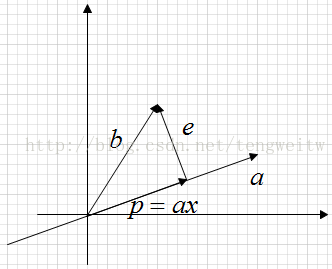
\includegraphics[width=0.7\linewidth]{math/img/1}  %插入的图,包括JPG,PNG,PDF,EPS等,放在源文件目录下
	\caption{向量b在向量a上的投影.}  %图片的名称
	\label{fig:mcmthesis-logo}   %标签,用作引用
\end{figure}
\noindent 图中,$\textit{\textbf{e}}=\textit{\textbf{b}}-\textit{\textbf{p}}=\textit{\textbf{b}}-x\textit{\textbf{a}}$,向量\textit{\textbf{e}}为投影残差\\
向量\textit{\textbf{a}}与向量\textit{\textbf{e}}垂直,\\ 
$\textit{\textbf{a}}^T\textit{\textbf{e}}=0 \longrightarrow \textit{\textbf{a}}^T(\textit{\textbf{b}}-x\textit{\textbf{a}})=0 \longrightarrow x\textit{\textbf{a}}^T\textit{\textbf{a}}=\textit{\textbf{a}}^T\textit{\textbf{b}} \longrightarrow x = \frac{\textbf{\textit{a}}^T\textbf{\textit{b}}}{\textbf{\textit{a}}^T\textbf{\textit{a}}}$\\
$x$是一个标量值,刻画了向量b投影到向量a上的长度。\\
\begin{center}
$\textbf{\textit{p}}=\textbf{\textit{a}}x = \textbf{\textit{a}}\frac{\textbf{\textit{a}}^T\textbf{\textit{b}}}{\textbf{\textit{a}}^T\textit{\textbf{a}}}$\\
\end{center}
\textbf{P}为投影矩阵,$\textbf{P}\textit{\textbf{b}}=\textit{\textbf{p}}$,则:
\begin{center}
$\textbf{P}=\frac{\textit{\textbf{a}}\textit{\textbf{a}}^T}{\textit{\textbf{a}}^T\textit{\textbf{a}}}$	
\end{center}


\subsection*{Gram-Schmidt正交化}

   
\chapter{DSO原理}

\section{残差形式}	
残差公式$r^k$是Host帧i到Target帧j上的匹配点的K的某个patch投影的residual:
\begin{equation} \label{eq:residual}
\begin{aligned} %等号对齐,但是会每一行都编号。 \begin{equation}则只编一个号
r_{ij}^k &= r^k(x \boxplus \xi_{0})\\
         &= I_{j}[p^{'}(T_{i},T_{j},d_{k},c)]-b_{j}-\frac{t_{j}e^{a_{j}}}{t_{i}e^{a_{i}}}(I_{i}(p^k)-b_{i}) \\ 
\end{aligned}
\end{equation}
其中
\begin{equation}
\begin{aligned} \label{eq:p}
p^{'} &= \pi(R\pi^{-1}(p,d_{p})+t)\\
&= \pi(T_{j}T_{i}^{-1}\pi^{-1}(p,d_{p}))
\end{aligned}
\end{equation}
而位姿的se(3)表示为
\begin{equation}
   T_{j}=exp(\hat{\xi}_{j}),T_{i}=exp(\hat{\xi}_{i})
\end{equation}
投影和反投影方程分别为
\begin{align}
	\pi(P)=(\frac{f_{x}P_{x}}{P_{z}}+c_{x},\frac{f_{y}P_{y}}{P_{z}}+c_{y})\\
	\pi^{-1}(P,d_{p})=(\frac{p_{x}-c_{x}d_{p}}{f_{x}},\frac{p_{y}-c_{y}d_{p}}{f_{y}},d_{p})
\end{align}
注意:\\
1、残差方程中,涉及到i、j两个时刻的pose。而基于feature point的slam中只于当前时刻的pose相关,将全局坐标系下面的point转换到当前帧下计算重投影误差。\\
2、考虑了亮度值的仿射变换a、b。\\

以上对应论文中的残差形式,而代码中涉及到更为细节,下面进行展开。
这里考虑在优化时有两个关键帧,一个称为Host,一个称为Target。取Host帧中的一个像素点:

\begin{equation}
	x_{H}=[u_{H},v_{H},1]_{H}^{T}\\
\end{equation}

其中$u_{H},v_{H}$为该点的像素坐标系,使用齐次坐标为了方便矩阵运算。同时,点的逆深度为:
\begin{equation}
\rho_{H}=\frac{1}{d_{H}}\\
\end{equation}

在不考虑亮度放射变换时,点p从Host帧i变换到到Target帧j上的过程为:
\begin{equation}
\begin{matrix}
    \overbrace{\rho_{T}^{-1} K^{-1} x_{T} =  T_{TW}}^{P_W}   \overbrace{T_{HW}^{-1} \frac{1}{\rho_{H}}K^{-1}x_{H}}^{P_W} \\ \\
	\underbrace{\rho_{T}^{-1} K_{-1} x_{T}}_{p_T} =  \underbrace{T_{TW}T_{HW}^{-1}}_{T_{TH}}  \underbrace{\frac{1}{\rho_{H}}K^{-1}x_{H}}_{p_H}
\end{matrix}
\end{equation}

将SE(3)形式展开
\begin{equation}
	T_{TH}=
	\left[ \begin{array}{cc}
	R_{TH} \quad t_{TH}\\
	0      \quad  1
	\end{array}
	\right]
\end{equation}
代入上式得:\\
\begin{equation}\label{eq:p1}
	x_{T} = \frac{\rho_{T}}{\rho_{H}}(KR_{TH}K^{-1}x_{H}+Kt_{TH}\rho_{H})
\end{equation}

\noindent \textbf{注:}
\begin{itemize}
  \item [1)] 公式中省略了齐次坐标和非齐次坐标的转换过程。推导时请自行脑补。
  \item [2)] 对于逆深度的操作,有些和常规习惯不同,但是代码中就是这样实现的,而且感觉挺方便的,后面会结合具体代码进行分析。
  \item [3)] 公式(\ref{eq:p})中的$p^{'}$表示一个投影过程,而(\ref{eq:p1})的$x_{H}$表示从Host中变换到Target后的一个点,二者实质是一样的。即(\ref{eq:p1})是(\ref{eq:p})
  的展开形式。
\end{itemize} 



%=========================================================================================================================
\section{参数形式}  %注意,不识别中文的标点符号"、",因此拆开写
涉及到的参数为$\xi_{i}$、$\xi_{j}$、$d$、$c$、$a_{i}$、$a{j}$、$b_{i}$、$b_{j}$。其中$\xi_{i}$、$\xi_{j}\in SE(3)$ 为两帧的外参,d为point在其host帧中的深度, $c\in R^4$为相机的内参,$a_{i},a{j},b_{i},b_{j}$分别为光照参数。 \\
\indent 按照Jacobian的结构可以分为2类,$T_{i}$、$T_{j}$、$d$、$c$= $(f_{x},f_{y},c_{x},c_{y})$为geometry参数$\delta_{geo}$,而$a_{i}$、$a_{j}$、$b_{i}$、$b_{j}$为photometric参数$\delta_{photo}$。\\
\indent 每个点以某一个pattern来构成,pattern形式见论文"Figure 4.\textbf{Residual pattern}"。按照层级,参数又可以分为全局属性$c$、帧属性$\xi_{i}$、$\xi_{j}$、$ab_{i}$、$ab_{j}$,点属性$d_{k_i}$(注意,这里是$i$,表示的是点在host帧下面的深度)。自变量中$d$的数量是最多。\\
\indent 同时,按照参数的来源的分类,即可以分为Host参数(下标为i,代码中表示为为h)和Target参数(下标为j,代码中表示为t)


%========================================================================================================================
\section{雅可比}
Jacobian定义为:
\begin{equation}
	J_{k}=\frac{\partial r^k((\delta+x)\boxplus\xi_0)}{\partial\delta}
\end{equation}
论文里,根据残差形式(\ref{eq:residual})将其划分为两部分
\begin{equation}
	J_{k}=[\underbrace{\frac{\partial I_j}{\partial p^{'}}}_{J_I} \underbrace{\frac{\partial p^{'}(\delta+x)\boxplus\xi)}{\partial\delta_{geo}}}_{J_{geo}}, \underbrace{\frac{\partial r_{k}((\delta+x)\boxplus x_0)}{\partial\delta_{photo}}}_{J_{photo}}]
\end{equation}
其中,$J_I=\frac{\partial I_j}{\partial p^{'}}=(\frac{\partial I_j}{\partial p_x^{'}},\frac{\partial I_j}{\partial p_y^{'}})\in R_{1x2}$是当前像素的的亮度的梯度值\\
在完整DSO中,雅可比由三部分组成:\\
图像雅可比$J_I$,即图像梯度;\\
几何雅可比$J_{geo}$,描述各量相对几何量,例如旋转和平移的变化率;\\
光度雅可比$J_{photo}$,描述各个量相对光度参数的雅可比;\\

\subsection{图像雅可比$J_I$}
$J_I=\frac{\partial I_j}{\partial p^{'}}=\frac{\partial I_j}{\partial x_{T}}$即图像的梯度

\subsection{几何雅可比$J_{geo}$}

\subsubsection{对pose求导}
几何部分包括相机的位姿和特征点的深度,需要对两部分求雅可比。\\
\indent 记$\xi_{T}$和$\xi_{H}$分别为$T_{TW}$、$T_{HW}$的李代数形式,位姿部分的雅可比:
\begin{equation}
	\frac{\partial x_{H}}{\partial \xi_{T}}=
	\left[	
	\begin{matrix}
		\rho_{T}f_{x} & 0 & -\rho_{T}uf_{x} & -uvf_{x} & (1+u^2)f_{x} & -vf_{x} \\
		0 & \rho_{T}f_{y} & -f_{y}\rho_{T}v & -(1+v^2)f_{y} & f_{y}uv & f_{y}u  
	\end{matrix}	
	\right]
\end{equation}

\begin{equation}
\frac{\partial x_{H}}{\partial \xi_{H}}= ????????
\end{equation}

\subsubsection{对逆深度求导}
再考虑对Host帧中的逆深度$\rho_{H}$的雅可比:
\begin{equation}
\frac{\partial x_T}{\partial \rho_H}=
\left[ \begin{matrix}
\frac{\partial x_{T}}{\partial u} \quad \frac{\partial x_{T}}{\partial v}
\end{matrix}
\right]
\left[
\begin{matrix}
\frac{\partial u}{\partial \rho_{H}}\\
\frac{\partial v}{\partial \rho_{H}}
\end{matrix}
\right]
\end{equation}

\subsubsection{对相机内参求导}





%========================================================================================================================
\section{边缘化}


\chapter{DSO代码分析--前端跟踪}

整个项目代码量比较大,文件很多。而且作者为了提高计算效率,优化相关的部分,很多中间结果共用,也没有采用开源的优化库ceres、gtsam等,所有部分纯手撸。而且还进行了SSE加速,也没使用OpenCV中的算法。因此,代码及其复杂,还涉及到分厂多的参数,这些参数与作者的使用调试经验强相关。
整个关键代码部分,可以分为三个部分:
\begin{itemize}
	\item  初始化
	\item  帧间跟踪
	\item  局部优化
\end{itemize} 
\paragraph{初始化} 作者在github的项目主页上说到,初始化并不是很鲁棒,用户可以自己实现自己的初始化操作。
\paragraph{帧间跟踪} 帧间跟踪主要是进行图像对齐,计算帧间的pose,类似基于特征点法计算H或者F分解得到Pose的过程,同时还要更新点的深度信息。
\paragraph{局部优化} 局部优化中做的事儿就有点儿多了,重头戏。


%===================================================
\section{标定矫正}


%===================================================
\section{系统初始化}


%===================================================
\section{帧间跟踪}	
\vspace{0.2em}
DSO中帧间跟踪时,只计算当前帧与前一个\textbf{关键帧}间的pose,即粗略跟踪。\\
\indent 完成粗跟踪的类是CoarseTracker,该类在FullSystem中共有两个对象,分别是coarseTracker\_forNewKF、coarseTracker。\\
二者的区别是:\\
\textbf{coarseTracker}:用于所有帧的跟踪,每一个非关键帧到来时,都计算相对于coarseTracker中保存的关键帧的相对pose。两个关键帧间的所有非关键帧使用的coarseTracker对象是同一个。\\
\textbf{coarseTracker\_forNewKF}:用于更新存储当前关键帧的信息。即当前帧是关键帧时,更新该对象,然后在下一帧(非关键帧)到来时,复制给coarseTracker对象。更新的信息包括refFrameID信息,在makeKeyFrame()函数中完成,且是在完成关键帧之后和边缘化之前。\\
\indent 新帧到来时,若coarseTracker\_forNewKF中的refFrameID比coarseTracker中的refFrameID大(因为其在前一关键帧中被更新,而coarseTracker中保存的还是前前关键帧),就将coarseTracker\_forNewKF赋给coarseTracker。若没有,coarseTracker维持之前的状态,即最后一个keyframe。更新过程只发生在关键帧及其下一帧中间。





%%%%%%%%%%%%%%%%%%%%%%%%%%%%%%%%%%%%%%%%%%%%%%%%%%%%%%%%%%%%%%%%%%%%%%%%%%%%%%%%%%%%%%%%%%%%%%%%%%%%%%%%%%%%%%%
%%%%%%%%%%%%%%%%%%%%%%%%%%%%%%%%%%%%%%%%%%%%%%%%%%%%%%%%%%%%%%%%%%%%%%%%%%%%%%%%%%%%%%%%%%%%%%%%%%%%%%%%%%%%%%%

\chapter{DSO代码分析--后端优化}
后端优化在makeKeyFrame()中,依次有十几项步骤:



%=================================================================================
\section{点的深度计算}
关键点的深度的计算都在后端完成,前端之负责计算两帧间的pose的初值。分为两步:
\begin{itemize}
	\item [1)] 通过深度滤波器更新点的深度范围,直到点的深度收敛,作为深度的初值。
	\item [2)] 在完成帧间pose的优化后,进一步优化点的深度值。
\end{itemize} 


\subsection{深度滤波}
通过深度滤波器完成深度范围的更新,在函数ImmaturePoint::traceOn()中,主要维持两个变量:idepth\_min、idepth\_min。将点投影到Target帧中,形成对应的两个点ptpMin、ptpMax,如果两个点的距离小于一定的阈值,则认为该点深度收敛:
\begin{lstlisting}[caption={  ImmaturePoint::traceOn()}]  
Vec3f pr = hostToFrame_KRKi * Vec3f(u,v, 1);
Vec3f ptpMin = pr + hostToFrame_Kt*idepth_min;		
.....
Vec3f ptpMax;
ptpMax = pr + hostToFrame_Kt*idepth_max;
......
if(!(uMax > 4 && vMax > 4 && uMax < wG[0]-5 && vMax < hG[0]-5))
{
  if(debugPrint) printf("OOB uMax  %f %f - %f %f!\n",u,v, uMax, vMax);
  lastTraceUV = Vec2f(-1,-1);
  lastTracePixelInterval=0;
  
  return lastTraceStatus = ImmaturePointStatus::IPS_OOB;
}
\end{lstlisting}  

\noindent 对深度进行深度更新:
\begin{equation}
\begin{aligned}
u-\delta e dx &= \frac{(pr + \rho_{min}Kt)[0]}{(pr + \rho_{min}Kt)[2]}\\
u+\delta e dx &= \frac{(pr + \rho_{max}Kt)[0]}{(pr + \rho_{max}Kt)[2]}
\end{aligned}
\end{equation}
式中,$pr=KR_{TH}K^{-1}*p_{H}$是点从Host帧中旋转到Target帧后的样子(即Point Rotation的简写),未考虑平移。平移和深度相关,深度相关的和前面重点强调的是一样的。
变形后得到代码中的形式:
\begin{equation}
\begin{aligned}
\rho_{min}  &= \frac{(pr[2]*(u-\delta e dx)-pr[0]}{(kt)[0] - (Kt)[2]*(u-\delta e dx)}\\
\rho_{max}  &= \frac{(pr[2]*(u+\delta e dx)-pr[0]}{(kt)[0] - (Kt)[2]*(u+\delta e dx)}
\end{aligned}
\end{equation}

\subsection{深度优化}
在优化时,会专门对深度进行优化


%==============================================================================================================
\section{Bundle Adjustment}
\indent 这一部分是整篇中最为核心的地方。作者将Hessian矩阵分为active、linear、marginal三部分。
在AccumulatedTopHessianSSE::addPoint()函数中,模板参数mode的值0、1、2分别表示active、linearized、marginalize。但是经测试linearized下面的实际部分并未执行,作者在逻辑中将其屏蔽掉了。
\subsection*{active部分}

\subsection*{marginal部分}

\section{边缘化}


\chapter{代码细节}
\section{比例因子}
代码中好多地方出现比例因子,这些因子作用是提高求解方程式 $$ H\bigtriangleup\!x=b $$的数值稳定性和精确度.\\
出现的地方:\\
1、方程求解的过程中\\
2、FrameHessian中\\


\end{document}
